% Template file for ICEAA13
%
\RequirePackage{ifpdf}
\documentclass{ICEAA-IEEE_APWC}
\usepackage{multirow}

\newcommand{\kvec}{{\bf k}}
\newcommand{\bvec}{{\bf b}}
\newcommand{\shat}{{\hat s}}
\newcommand{\kpr}{{k_\perp}}
\newcommand{\kvpr}{{\kvec_\perp}}
\newcommand{\kpar}{{k_\parallel}}
\newcommand{\AI}{{\langle\tilde A*\tilde I\rangle}}
\newcommand{\AItau}{{\AI(\tau)}}
\newcommand{\hMpci}{{h~{\rm Mpc}^{-1}}}
\newcommand{\inch}{$^{\prime\prime}$}
\newcommand{\foot}{$^{\prime}$}
\renewcommand{\deg}{^\circ}

% In order to produce the pdf document for paper submission either:
% a) process with pdfLaTeX, or
% b) process with LaTeX, dvips, ps2pdf
% In both cases comment out the document class option as indicated above

\newcommand\aj{AJ}%
          % Astronomical Journal
\newcommand\actaa{\ref@jnl{Acta Astron.}}%
  % Acta Astronomica
\newcommand\araa{\ref@jnl{ARA\&A}}%
          % Annual Review of Astron and Astrophys
\newcommand\apj{ApJ}%
          % Astrophysical Journal
\newcommand\apjl{\ref@jnl{ApJ}}%
          % Astrophysical Journal, Letters
\newcommand\apjs{\ref@jnl{ApJS}}%
          % Astrophysical Journal, Supplement
\newcommand\ao{\ref@jnl{Appl.~Opt.}}%
          % Applied Optics
\newcommand\apss{\ref@jnl{Ap\&SS}}%
          % Astrophysics and Space Science
\newcommand\aap{\ref@jnl{A\&A}}%
          % Astronomy and Astrophysics
\newcommand\aapr{\ref@jnl{A\&A~Rev.}}%
          % Astronomy and Astrophysics Reviews
\newcommand\aaps{\ref@jnl{A\&AS}}%
          % Astronomy and Astrophysics, Supplement
\newcommand\icarus{\ref@jnl{Icarus}}%
  % Icarus
\newcommand\mnras{\ref@jnl{MNRAS}}%
          % Monthly Notices of the RAS
\newcommand\prc{\ref@jnl{Phys.~Rev.~C}}%
          % Physical Review C
\newcommand\prd{\ref@jnl{Phys.~Rev.~D}}%
          % Physical Review D
\newcommand\pre{\ref@jnl{Phys.~Rev.~E}}%
          % Physical Review E
\newcommand\prl{\ref@jnl{Phys.~Rev.~Lett.}}%
          % Physical Review Letters
\newcommand\pasa{\ref@jnl{PASA}}%
  % Publications of the Astron. Soc. of Australia
\newcommand\pasp{\ref@jnl{PASP}}%
          % Publications of the ASP


\title{The Hydrogen Epoch of Reionization Array (HERA)}

% Use \thanks{} for each affiliation.
% If the authors have the same affiliation, use \thanks[n] to
% refer to the same affiliation of the n:th \thanks command
\author{D. R. DeBoer\thanks{Radio Astronomy Laboratory, University of California, Berkeley, CA 94720, USA, e-mail: ddeboer@berkeley.edu}, 
on behalf of the HERA collaboration
}
\begin{document}
\maketitle


\begin{abstract}
The Hydrogen Epoch of Reionization Array (HERA http://reionization.org) is a staged experiment that uses the unique properties of the 21-cm line from neutral hydrogen to probe the Epoch of Reionization (EOR). During this epoch, roughly 0.3 - 1 billion years after the Big Bang, the first galaxies and black holes heated and reionized the early Universe. Direct observation of the large scale structure of reionization and its evolution with time will have a profound impact on our understanding of the birth of the first galaxies and black holes, their influence on the intergalactic medium (IGM), and cosmology.  This paper will provide an overview of the project and describe the design of the HERA receiving element.

\end{abstract}

\section{Introduction}
\label{sec:intro}
We have garnered a deep understanding of the large scale structure of the very early Universe by observing the faint afterglow of the cosmic microwave background (CMB).  The CMB signal arises due to the recombination of hydrogen gas which allows the radiation to stream forth.  It represents one slice in time when the faint imprint of the nearly homogeneous inflationary Universe may be seen.

We also have a good understanding of the complicated structure and denizens of our current Universe.  In between however, we have very little information of how our Universe evolved to its current structure.  It is as if we have one detailed snapshot from one day in the first days of our baby's life, and then a Facebook page of our child as a young adult with very little in between except faint rumors and a headline or two.

This intervening period has essentially four phases which may be called the Dark Ages, the Cosmic Dawn, the Epoch of Reionization (EOR) and the Rise of the Galaxies.  The time of the Cosmic Dawn saw the first large-scale gravitational collapse of structures, which eventually heated up the neutral intergalactic hydrogen gas until it again ionized.  This phase change is called the Epoch of Reionization and it represents the last phase change of the Universe as a body.  We may observe this epoch over its extent by observing the red-shifted hydrogen gas.  In our analogy, this is akin to following our child's activities and growth through a good part of their formative years.

Detecting, characterizing and ultimately imaging the Epoch of Reionization is a key goal for the astronomy and astrophysics community. There are many references on the theoretical, instrumental and observational foundations, see for example one of the latest instrument papers and references therein ({\em e.g.} {\cite{2015arXiv150206016A}}).  Current projects (PAPER (http://eor.berkeley.edu), MWA (http://mwatelescope.org), LOFAR (http://www.lofar.org)) are striving to make the first detection of the statistical power spectrum of the signal, however current best limits still fall above even optimistic predictions of its intrinsic strength.  While these projects are still taking data, it is recognized that an optimized array based on our new understanding of the signal characteristics is needed to make a strong detection and begin to characterize this signal over multiple scales and redshifts.  These results would also inform design elements for the Square Kilometer Array (http://www.skatelescope.org).

The Hydrogen Epoch of Reionization Array (HERA http://reionization.org) is a staged experiment that uses the unique properties of the 21-cm line from neutral hydrogen to probe the EOR, roughly 0.3 - 1 billion years after the Big Bang. Direct observation of the large scale structure of reionization and its evolution with time will have a profound impact on our understanding of the birth of the first galaxies and black holes, their influence on the intergalactic medium (IGM), and cosmology.

\begin{figure}[t]
\centerline{
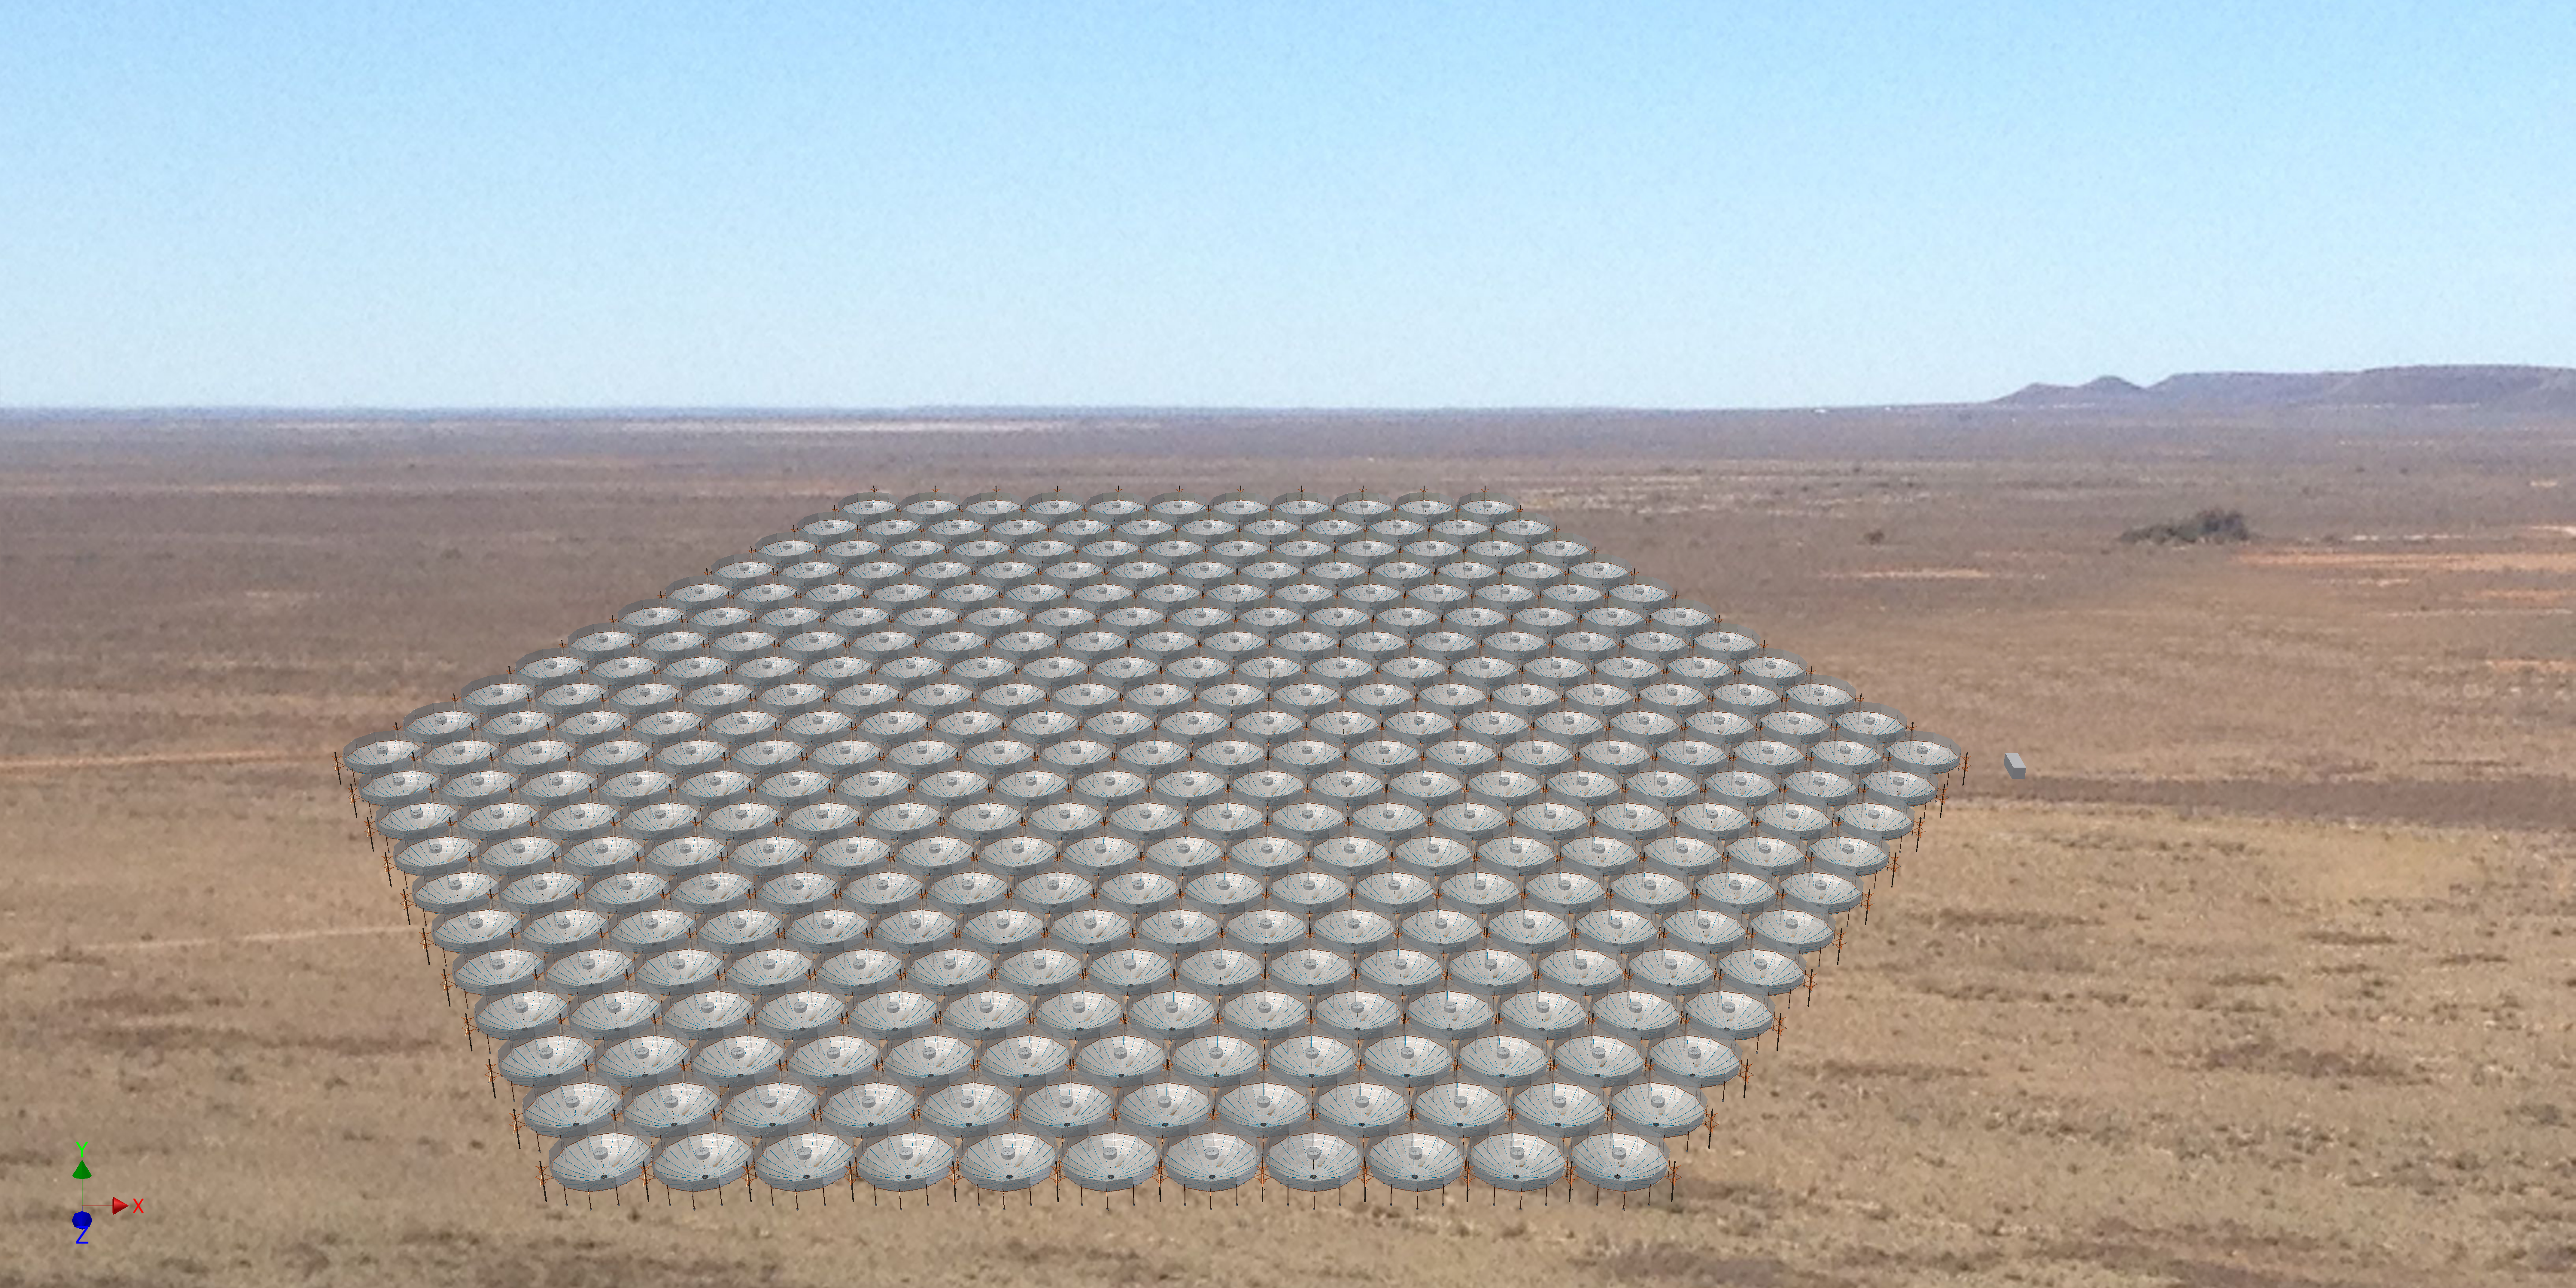
\includegraphics[width=7.5cm]{hera331_Bpers.png} }
\caption{\small Perspective cartoon of the 331-element core within a 305-meter circle.
\label{fig:config}}
\end{figure}

HERA has been funded under the US National Science Foundation's Mid-Scale Innovations Program to begin building elements optimized for robust power spectrum detection.  The key is to produce inexpensive collecting area optimized for the spatial scales needed to detect the EOR.  This has resulted in a close-packed array of transit 14-meter dishes (Fig. \ref{fig:config}), with the first elements currently under construction at the South African Karoo Astronomy Reserve, the current location of the Donald C. Backer Precision Array to Probe the Epoch of Reionization (PAPER) array.

Beginning with the current NSF funding, HERA will rollout in a staged deployment.  The first phase extending to August 2016 will deploy 37 elements that will test the HERA element design for performance and manufacturability at location.  These 37 elements will more than double the sensitivity of the 128-element PAPER array.  The next phase extending into 2018 will build out to 127 elements, which should provide a very robust detection of the EOR signal.  Finally, extending into 2020, HERA will build out to 352 elements to further EOR science as a function of redshift and spatial scale, potentially producing the first images of the EOR.

HERA is a collaboration of the following partner institutions:  Arizona State University, University of California Berkeley, University of California Los Angeles, University of Cambridge, University of KwaZulu Natal, Massachusetts Institute of Technology, National Radio Astronomy Observatory, University of Pennsylvania, SKA-South Africa, and
University of Washington.

\section{Measuring the EOR}
\label{sec:eormeas}
Due to the expansion of the Universe, we can identify and measure the early Universe via the red-shift of spectral lines.  The hydrogen hyperfine transition at a rest frequency of 1420 MHz is a key spectral line due to the ubiquity of hydrogen and, being a ``forbidden'' transition, the optical depth lets us see through the entire Universe back almost to the period of recombination.  Frequency therefore equates to a volume along the site of the telescope as well as in dating when the event occurred. 

Initial measurements of the EOR strive to measure a statistical power spectrum of the signal since the nature of the reionization process should have a specific spatial signature.  The goal is therefore to measure a range of aggregate spatial scales on the sky, rather than to image the signal directly.  Imaging does remain an ultimate goal to fully understand the process, however we will need a greater understanding of its properties to achieve this more difficult goal.  

Given that the response of an interferometer natively measures the power in Fourier modes of the sky within its beam, we see that it is a natural instrument to use for this measurement.  We can essentially relate the sky power spectrum mode ${\hat P}(\kvec)$ to an interferometer baseline visibility ${\tilde V}(\bvec)$, which is the equivalent of the (complex) fringe pattern in a double slit experiment (see {\em e.g.} \cite{2012ApJ...756..165P}):
\begin{equation}
{\hat P}(\kvec) \approx \left(\frac{X^2Y}{4k_B^2}\right) \frac{{\tilde V}^2(\bvec)}{\Omega_b B/ \lambda^4} 
\end{equation}
where $X$ and $Y$ are cosmological parameters relating angular size and spectral frequency to cosmic volumes, $\Omega_b$ is the integrated squared beam response, $B$ is the effective bandwidth, $\lambda$ is the observation wavelength, and $k_B$ is Boltzmann's constant.  The terms not in parentheses are instrumental terms, as opposed to constants and cosmological parameters.

Though the desired measurement is over a 3-D volume, it is instructive to split it into two components,  $\kvec =  \kvpr + \kpar{\hat {\bf z}}$ where $\kpr$ is determined by the antenna baseline and $\kpar$ by the frequency.  This is useful since it allows us to split out the chromatic response of the interferometer and isolate a phase space where foreground sources ({\em i.e.} everything not the EOR) contaminate the signal of interest from where they don't.  This contaminated phase space may be shown to be a wedge-shaped region in $\kpr$:$\kpar$ space:
\begin{equation}
|\kpar| \le \frac{X\lambda}{Yc}\kpr + \frac{S}{Y}
\end{equation}
where $c$ is the speed of light and $S$ is a parameter accounting for offsets related to the combined spectral smoothness of the foregrounds and the antenna response.  
A key issue to measuring the EOR power spectrum is to understand and minimize such effects.  For an analytical derivation, see \cite{2012ApJ...756..165P,vedantham_et_al2012,liu_et_al2014b},  in simulation see \cite{datta_et_al2010,hazelton_et_al2013} and for observations
\cite{2013ApJ...768L..36P,2015arXiv150601026P,2014ApJ...788..106P,2015arXiv150206016A}.

\section{HERA System}
\label{sec:system}
HERA will operate between 70 MHz and 220 MHz, however the first phases (up to 127 elements) will operate within the current PAPER bandwidth of 110-190 MHz.  The full band is directly sampled and correlated, making for a very simple signal path requiring only gain.  Initially, the exact PAPER signal chain will be used, which brings the RF back to a central container on coaxial cable where it is digitized and processed.  A new modular digitizer (Smart Network ADC Processor, or SNAP) has been developed that will be deployed in the field and will shorten the amount of RF cable.  The digitized signal will be conveyed back to a central building for processing via 10 Gbit ethernet over fiber-optic cable.   The SNAP board is being developed as part of the CASPER suite of hardware components (https://casper.berkeley.edu/wiki/DAB-HERALD).  A simple block diagram of the two-phase system is shown in Fig. \ref{fig:system}.

\begin{figure}[t]
\centerline{
\includegraphics[width=5.5cm]{system.png} }
\caption{\small High-level block diagram of the HERA system.  The dashed lines indicate the first phase while solid are the final design.  Black lines are coaxial cable and orange are ethernet over fiber.
\label{fig:system}}
\end{figure}

The configuration is optimized for power spectrum detections, which favors as large of a fill-factor as possible.  The configuration is therefore a packed hexagonal array with a 14.6-meter pitch with a 14-meter antenna (see Fig \ref{fig:config}).  Additionally, there will be 21 outriggers out to 1.2km to improve the resolution 

%\begin{table}[htpb]
%\centerline{
%\begin{tabular}{|l||c|c||c|c||}\hline
% \multirow{2}{*}{Instrument}                 & \multicolumn{2}{|c|}{Avoidance} & \multicolumn{2}{|c|}{Subtraction} \\ \cline{2-5}
%                      & Drift  & Track  & Drift  & Track \\ \hline
%PAPER 128  &  1.56  &  -  &  4.46  &  - \\ \hline
%MWA 128      &  0.66  & 0.86  &  2.50  &  3.15 \\ \hline
%LOFAR (core) & 0.70  & 1.90  & 7.48  &  12.22 \\ \hline \hline
%HERA 37         & 5.67  &  -  & 15.46   &  - \\ \hline
%HERA 331       & 38.75 & -  &  111.69  &  - \\ \hline
%MWA 256         &2.40   &  2.81  &  8.28  & 9.64 \\ \hline
%SKA1 Low      &21.23   & 26.92  & 139.07  & 115.13 \\ \hline
%\end{tabular}}
%\caption{\small Parameters and their values; units are spaced from the
%corresponding measure by an unbreakable thin space and should
%always be in upright font.\label{tab:sensitivity}}
%\end{table}

\section{HERA Element}
\label{sec:element}
The design of the HERA element is discussed in \cite{heraMemo5}.  The design principles are three-fold:
\begin{itemize}
\item optimize for the delay-spectrum technique of measuring the EOR power spectrum,
\item minimize costs, and
\item the experiment has a limited lifetime of about five years.
\end{itemize}
The first item primarily means that chromatic effects corresponding to delays appropriate for the measurement described above must be below the expected signal level, which essentially determines the focal length.  The second item constrains the diameter and element count, as well as the focal length over diameter ratio ($f/D$), based on a cost function and maximizing sensitivity per element.  And the third items constrains the construction materials and methods and the operational model.

The approach used first sets a specification on the magnitude of the reflections within the dish on the delays of interest.  Reference \cite{heraMemo5} derives this to be that the reflections must be down by 60 dB on timescales greater then 60 nanoseconds.  
Next, using a feed pattern based on the existing PAPER dipole antenna and a fairly complete analytical model of a prime focus antenna, the effective area was found to be maximized for $f/D \approx 0.32$.  Figure \ref{fig:costfig} shows the vertex/feed round-trip travel times for one, two and three reflections with the 60 ns timescale indicated by the black dashed line. 

To determine the optimal diameter, full system costings were done on a range of diameter sizes from 5m - 25m, where the total number was constrained to keep constant sensitivity for this measurement, which is shown in Figure \ref{fig:costfig}.  By assuming canonical values of 331 14-meter antennas, the number of elements needed for a given diameter to match the sensitivity is
\begin{equation}
N_a = 26918D_a^{-\frac{5}{3}}
\end{equation}
Figure \ref{fig:costfig} shows the resulting normalized system cost/performance-curve, which becomes quite flat for diameters greater than about 14m, which also happens to be the diameter where two reflections between the feed and vertex coincide with the 60 ns specification.  An addition high-level analysis of reflection coefficients within the structure also indicate that a diameter of less than 15 meters is preferred.  The diameter of 14 meters was therefore chosen for the element.

\begin{figure}[t]
\centerline{
\includegraphics[width=7.5cm]{costfig.png} 
}
\caption{\small Costing model for a fixed sensitivity system as a function of diameter (thick blue line and left axis) as well as the round-trip delay for 1,2 and 3 feed-vertex trips (dashed red lines and right axis).  The 60 ns spec is indicated by the horizontal dash line, and the two-trip intersection at about 14-meter is the vertical dashed line.
\label{fig:costfig}}
\end{figure}

A full-sized prototype of this system was built and measured using a network analyzer in time-domain mode, which meets the ``60 by 60 '' specification (Fig \ref{fig:refl}). (\cite{heraMemo5}).

\begin{figure}[t]
\centerline{
\includegraphics[width=7.5cm]{reflections.png} 
}
\caption{\small Network analyzer measurements of reflected power versus delay time of the full-size HERA prototype.
\label{fig:refl}}
\end{figure}

\section{Conclusion}
A system design meeting the above design principles was presented, which comprises 331 14-meter elements in a compact hexagonal grid and 21 outriggers out to a 1.2km maximum baseline.  HERA uses the demonstrated foreground avoidance technique and should provide a very robust detection of the EOR signal.  Additional work will continue on HERA and other arrays to get the first detection as well as to perfect techniques allowing us to get to the other spatial scales and image the EOR.  Figure \ref{fig:eorsense} compares the sensitivity of existing arrays (left of the thick vertical line) using the different techniques, along with future HERA and SKA arrays.  HERA has the strong potential to get a robust detection in the near-term and characterize the EOR and signal processing to feed into the SKA to get a more complete picture of this period in the life of our early Universe.

\begin{figure}[t]
\centerline{
\includegraphics[width=7.5cm]{eorsens.png} 
}
\caption{\small Sensitivity calculations for present and future arrays  (separated by the vertical thick black line) investigating the EOR.
The arrays are mentioned in Sec. \ref{sec:intro}.  The four bars per array refer to different observing and analysis techniques.  The "avoidance" 
methods are largely demonstrated while the "subtraction" ones are still under development.  Note that PAPER/HERA do not track.
\label{fig:eorsense}}
\end{figure}
\section*{Acknowledgments}
This material is based upon work supported by the National Science Foundation Graduate Research Fellowship under Grant No. 1440343.
\bibliographystyle{plain}
\bibliography{mybibdesk}

\end{document}
